%%%%%%%%%%%%%%%%%%%%%%%%%%%%%%%%%%%%%%%%%%%%%%%%%%%%%%%%%%%%%%%%%%%%%%%
% Info
%%%%%%%%%%%%%%%%%%%%%%%%%%%%%%%%%%%%%%%%%%%%%%%%%%%%%%%%%%%%%%%%%%%%%%%
% Author: Louis Pahlavi
% Email:  louis.pahlavi@mail.utoronto.ca

% This is my personal resume. All the document setup is made inside the
% "Resume" template.

%%%%%%%%%%%%%%%%%%%%%%%%%%%%%%%%%%%%%%%%%%%%%%%%%%%%%%%%%%%%%%%%%%%%%%%
% General setup
%%%%%%%%%%%%%%%%%%%%%%%%%%%%%%%%%%%%%%%%%%%%%%%%%%%%%%%%%%%%%%%%%%%%%%%
\documentclass{ResumeTemplate}
\usepackage{tabularx}
\usepackage{graphicx}

%%%%%%%%%%%%%%%%%%%%%%%%%%%%%%%%%%%%%%%%%%%%%%%%%%%%%%%%%%%%%%%%%%%%%%%
% Document
%%%%%%%%%%%%%%%%%%%%%%%%%%%%%%%%%%%%%%%%%%%%%%%%%%%%%%%%%%%%%%%%%%%%%%%
\begin{document}
	
	%%%%%%%%%%%%%%%%%%%%%%%%%%%%%%%%%%%%%%%%%%%%%%%%%%%%%%%%%%%%%%%%%%%
	% Title and headers
	%%%%%%%%%%%%%%%%%%%%%%%%%%%%%%%%%%%%%%%%%%%%%%%%%%%%%%%%%%%%%%%%%%%

	\centering\name{Louis L. W. D. Pahlavi}
	\contact{106 Wineva Ave}{Toronto, ON, Canada}{M4E 2T2}{+1-(647)-909-5487}{louis.pahlavi@mail.utoronto.ca}

	\subsubsection{~}

	\noindent\begin{minipage}[c]{0.75\linewidth} 
	
	\section{PERSONAL DETAILS}
	
	\noindent\begin{tabularx}{\linewidth}{>{\bfseries}lX}
	    Website & \href{https:\\lpahlavi.github.io}{lpahlavi.github.io} \\
	    Nationality & French, Canadian \\
	    Languages & French (native), English (native), Italian (fluent), German (intermediate) \\
	\end{tabularx}

	\section{TECHNICAL SKILLS}
	\raggedright
	\begin{itemize}[noitemsep, leftmargin=*]
		\item \textbf{Programming Languages:} Python, C/C++,  MATLAB, Java \\
		\item \textbf{Software and CAD:} Unix, Git, Jira, Gerrit, Simulink, Tensorflow, Qt, LaTeX
	\end{itemize}

	\end{minipage}
	\noindent\begin{minipage}[c]{0.2\linewidth}
		\centering
		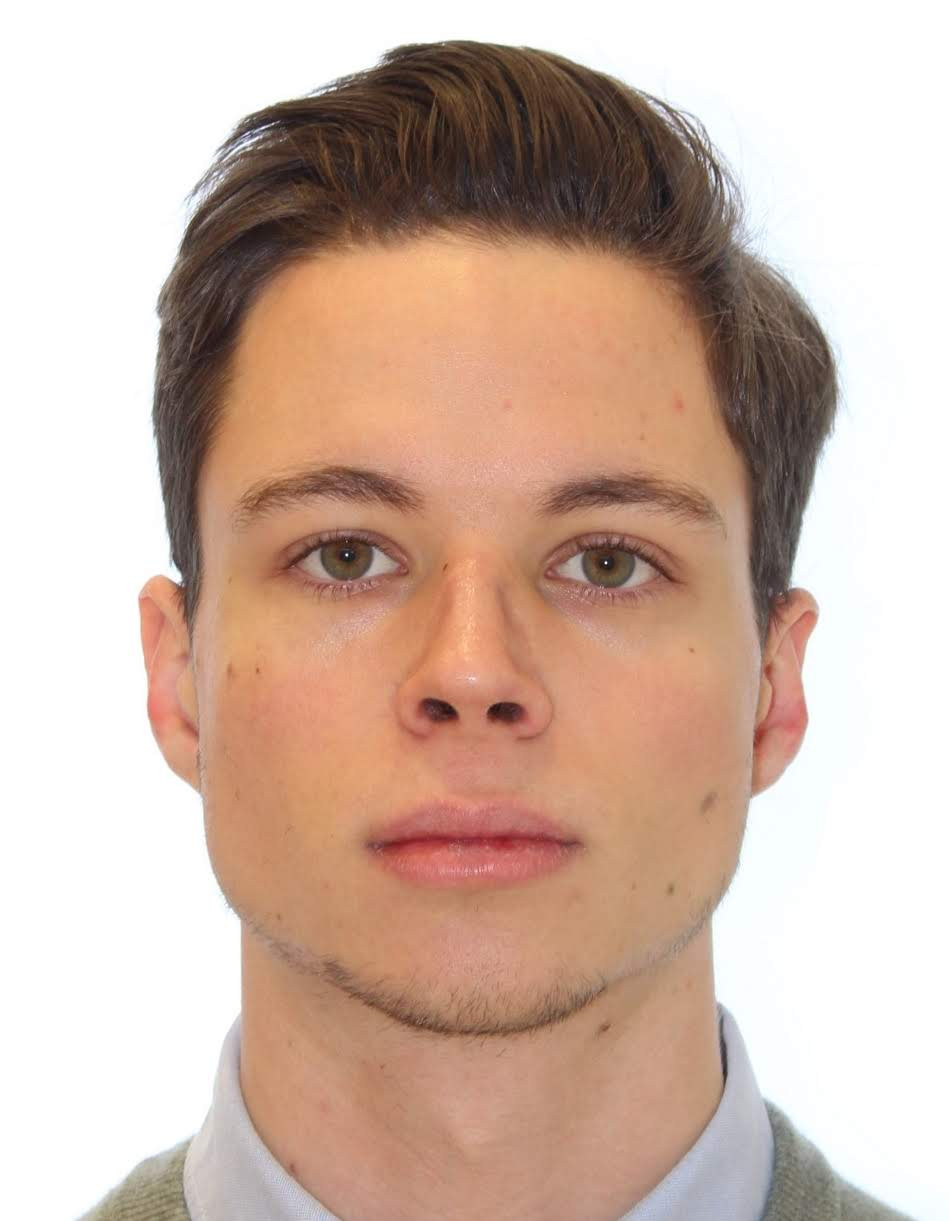
\includegraphics[width=0.9\linewidth]{me}
	\end{minipage}
	
	%%%%%%%%%%%%%%%%%%%%%%%%%%%%%%%%%%%%%%%%%%%%%%%%%%%%%%%%%%%%%%%%%%%
	% Education
	%%%%%%%%%%%%%%%%%%%%%%%%%%%%%%%%%%%%%%%%%%%%%%%%%%%%%%%%%%%%%%%%%%%
	\section{EDUCATION}
	
	\datedsubsection{University of Toronto, BASc in Computer Engineering}{September 2014--April 2019}
	\workitemsfour
	{Minor in Robotics and Mechatronics}
	{Final Project: \textit{Distributed Formation Control of a Swarm of Unicycles}}
	{16 month professional internship between third and fourth years of studies}
	{Latest term 92.1\% average (ranked 4 out of 173), 3.86/4.00 cumulative GPA}
	
	%%%%%%%%%%%%%%%%%%%%%%%%%%%%%%%%%%%%%%%%%%%%%%%%%%%%%%%%%%%%%%%%%%%
	% Education
	%%%%%%%%%%%%%%%%%%%%%%%%%%%%%%%%%%%%%%%%%%%%%%%%%%%%%%%%%%%%%%%%%%%
	\section{RESEARCH AND INDUSTRY EXPERIENCE}
	
	\position{Systems and Control Engineering Intern}{May 2017--August 2018}{\href{https://veritystudios.com/}{Verity Studios AG}}

	\workitemsthree
	{Worked on improving the onboard control algorithms of swarms of quadcopters implemented in C++.}
	{Evaluated and characterized flight performance and effectiveness of calibration routines using Python.}
	{Serviced entertainment drone show systems overseas and oversaw flight operations for several weeks.}
	
	\position{Researcher}{May 2016--August 2016}{\href{http://www.lbb.ethz.ch/}{ETH Z{\"u}rich Laboratory for Biosensors and Bioelectronics (LBB)}}
	
	\workitemstwo
	{Developed the control and image processing software for a biosensor measuring protein interactions.}
	{Created a Graphical User Interface using Qt to control the actuators and interface them with various sensors.}
	
	\position{Researcher}{May 2015--September 2015}{\href{http://www.waves.utoronto.ca/prof/svhum/}{University of Toronto Reconfigurable Antenna Laboratory}}

	\workitemstwo
	{Designed and simulated the early prototypes of a deployable antenna mounted on the NORSAT-2 maritime communications satellite (launched in 2017) in collaboration with the European Space Agency.}
	{Created a MATLAB simulation to model a satellite's orbit and predict antenna radiation intensity on the surface of the Earth. Worked on antenna synthesis to find an antenna array for a given desired coverage area.}
	
	%%%%%%%%%%%%%%%%%%%%%%%%%%%%%%%%%%%%%%%%%%%%%%%%%%%%%%%%%%%%%%%%%%%
	% Projects and Teaching
	%%%%%%%%%%%%%%%%%%%%%%%%%%%%%%%%%%%%%%%%%%%%%%%%%%%%%%%%%%%%%%%%%%%
	\section{PROJECTS}
	
	\position{Capstone Team Lead}{September 2018--April 2019}{\href{https://www.engineering.utoronto.ca/}{University of Toronto Faculty of Engineering}}

	\workitemsthree
	{Implementing a fully distributed algorithm for the formation control of a swarm of wheeled robots in C++.}
	{Responsible for the design of the communication interfaces between onboard modules in C++ and Python.}
	{Developed a Python simulation framework to test and tune the control algorithms. }
	
	\position{Wireless Communications Lead}{September 2014--June 2016}{\href{https://www.utat.ca/space-systems/}{University of Toronto Aerospace Team}}

	\workitemstwo
	{Designed, built and tested the antenna and communication module PCB, on a student-built nano-satellite.}
	{Presented our design at several Product Design Reviews and the Critical Design Review in Vancouver.}
	
	%%%%%%%%%%%%%%%%%%%%%%%%%%%%%%%%%%%%%%%%%%%%%%%%%%%%%%%%%%%%%%%%%%%
	% Awards and Scholarships
	%%%%%%%%%%%%%%%%%%%%%%%%%%%%%%%%%%%%%%%%%%%%%%%%%%%%%%%%%%%%%%%%%%%
	\section{SCHOLARSHIPS AND AWARDS}	
	\begin{itemize}[noitemsep, leftmargin=*]
		\item \textbf{Faculty of Applied Science and Engineering Dean's Honours List} \hfill 2014--Present
		\item \textbf{Gordon R. Slemon Scholarship} -- Awarded for engineering design and academic excellence \hfill 2016
		\item \textbf{University of Toronto International Exchange Bursary} \hfill 2016
		\item \textbf{University of Toronto Centre for International Exchange Award} \hfill 2016
		\item \textbf{Royal Canadian Air Cadet Glider and Power Pilot Scholarships} \hfill 2013, 2014\vspace*{-\baselineskip}
	\end{itemize}

\end{document}